\documentclass[10pt,a4paper,notitlepage]{report}
\usepackage[utf8]{inputenc}
\usepackage[english]{babel}
\usepackage{amsmath}
\usepackage{amsfonts}
\usepackage{amssymb}
\usepackage{hyperref}
\usepackage{graphicx}
\usepackage{listings}
\usepackage{lmodern}
\usepackage{fourier}
\usepackage[left=2cm,right=2cm,top=2cm,bottom=2cm]{geometry}
\author{Steven Huerta}
\title{QGroundControl Installation}
\begin{document}
\maketitle
\section*{Intro}
\noindent \textbf{DISCLAIMER:} This installation walkthrough and the software is owed to the hard work and efforts of Lorenz Meier ,as well as the developers and maintainers of QGroundControl(credits found \href{http://qgroundcontrol.org/credits}{here}).\\

\noindent These instructions can be found at \hspace{2mm} \url{http://qgroundcontrol.org/users/start}\\

\section*{LINUX INSTALL: Ubuntu 14.04}
\begin{enumerate}
\item Download and install Qt. Instruction found \href{https://wiki.qt.io/Install_Qt_5_on_Ubuntu}{here}.
\item Install some additional dependencies
\begin{lstlisting}[language=bash]
$ sudo apt-get install espeak libespeak-dev libudev-dev libsdl1.2-dev
\end{lstlisting}
\item Find someplace to either clone the repository and: 
\begin{lstlisting}[language=bash]
$ git clone --recursive https://github.com/mavlink/qgroundcontrol.git
\end{lstlisting}
You can also just download the \href{http://qgroundcontrol.s3.amazonaws.com/master/qgroundcontrol.tar.bz2?dl=0}{tar file}.
\item Now build the application by launching Qt Creator and opening qgroundcontrol.pro
\item After it is done building, you can run the application and QGroundControl will start(Fig.~\ref{fig:gcs}).
\end{enumerate}

\begin{figure}[h]
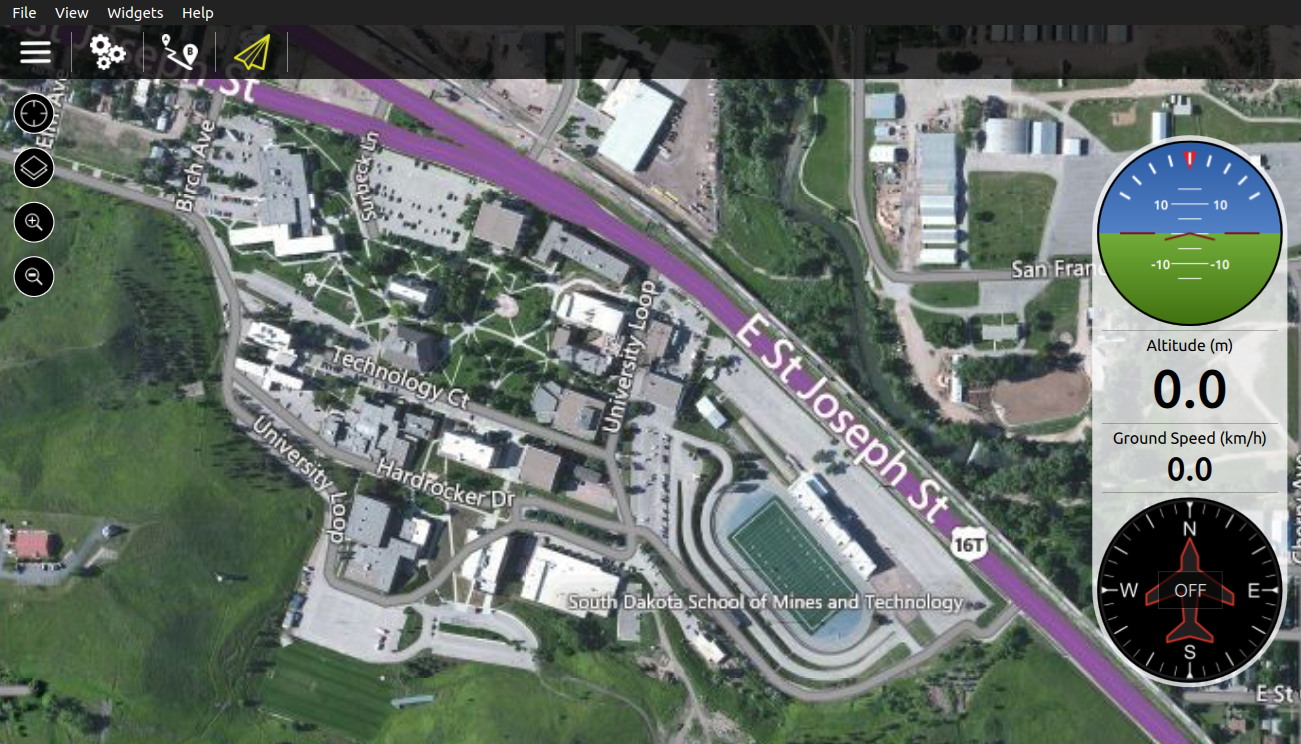
\includegraphics[scale=.35]{qgroundcontrol.png}
\caption{QGroundControl}
\label{fig:gcs}
\end{figure}

\section*{Running the GCS}
\begin{enumerate}
\item Run the executable generated by the building of the project. If you are still using Qt Creator, you can run the project and the application will launch.
\item If there are possible connections, a connect button should appear in the top right corner of the application.
\item To generate missions, with or without a connection, you can select the + sign in on the left side of the GUI. The first mission generated will be take-off by default(Fig.~\ref{fig:mission}). You can add additional waypoints and other commands by selecting the + button again. You can also change any of the already selected missions by selecting the mission and then selecting a new mission point from a drop down menu. 
\end{enumerate}


\begin{figure}[h]
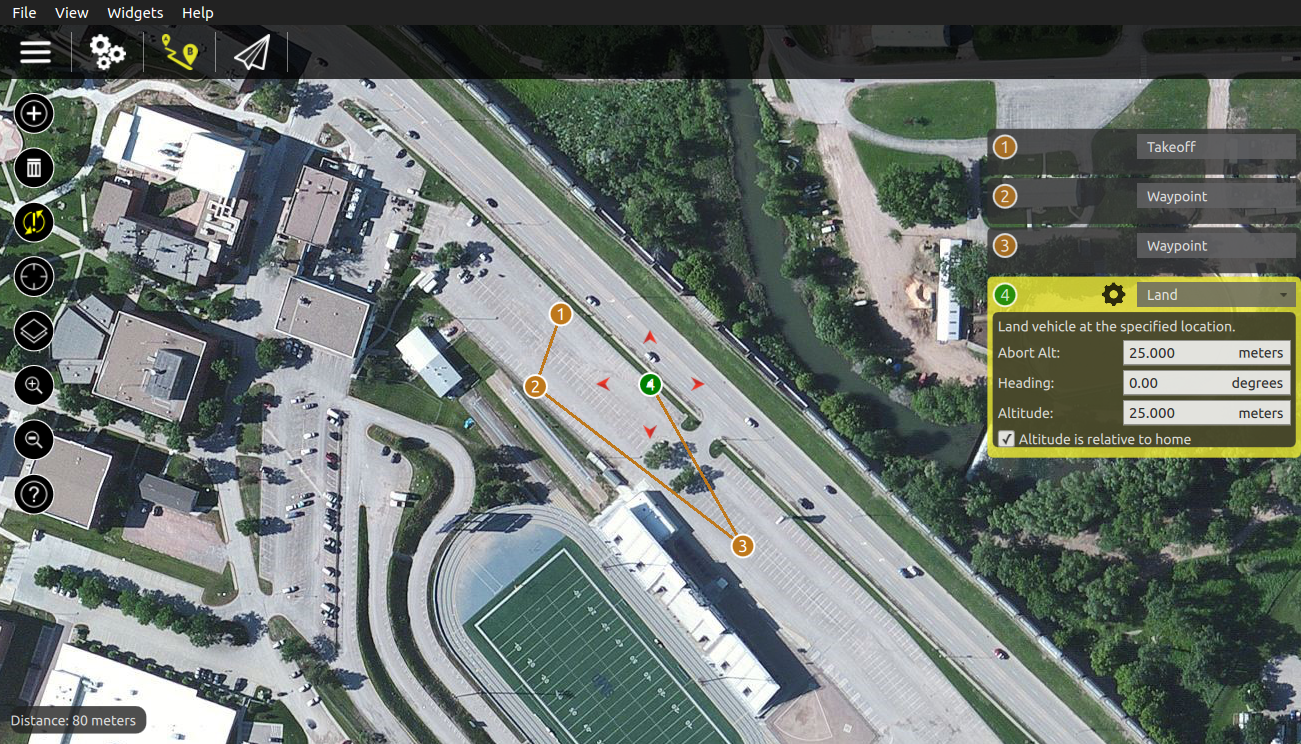
\includegraphics[scale=.35]{mission.png}
\caption{GCS with sample missions}
\label{fig:mission}
\end{figure}

\end{document}